\documentclass[14pt]{extarticle} 
\usepackage{amsmath,mathtools,amsfonts,amsthm,amssymb,hyperref}
\usepackage{wasysym,geometry,bussproofs,latexsym,parskip,bookmark}
\usepackage{mathtools,float}
\newtheorem{defn}{Definition}
\newtheorem{thm}{Theorem}
\newtheorem{claim}{Claim}
\newtheorem{lemma}{Lemma}
\hypersetup{colorlinks,allcolors=blue,linktoc=all}
\geometry{a4paper} 
\geometry{margin=0.5in}
\title{Math for CS 2015/2019 solutions to ``In-Class Problems Week 10, Fri. (Session 25)''}
\author{https://github.com/spamegg1}
\begin{document}
\maketitle
\tableofcontents

\section{Problem 1}
\subsection{(a)}
How many of the billion numbers in the range from 1 to 109 contain the digit 1? (Hint: How many don’t?)
\begin{proof}
We can count up how many do not contain the digit 1 and subtract. So (total number) - (number without 1’s) = $10^9 -(9^9 -1) = 612,579,512$ (the -1 is for 0 which is not in our range).
\end{proof}

\subsection{(b)}
There are 20 books arranged in a row on a shelf. Describe a bijection between ways of choosing 6 of these books so that no two adjacent books are selected and 15-bit strings with exactly 6 ones.
\begin{proof}
A selection of six among twenty books on a shelf corresponds in an obvious way to a 20-bit string with exactly six 1’s. For example, the 20-bit string with 1’s in exactly the 3rd, 4th, 5th, 10th, 19th and 20th positions corresponds to selecting 3rd, 4th, 5th, 10th, 19th and 20th books on the shelf.

So the problem reduces to finding a bijection between 20-bit strings with six nonadjacent 1’s and 15-bit strings with six 1’s.

But in a string $s$ with six nonadjacent 1’s, all but the last 1 must have a 0 to its right. So we can map $s$ to a string with six 1’s and five fewer 0’s by erasing the 0’s immediately to the right of each of the first five 1’s. For example, erasing the underlined 0’s in the 20-bit string $0001\underline{0}1\underline{0}01\underline{0}1\underline{0}00001\underline{0}10$ yields the 15-bit string 000110110000110.

This map is a bijection because given any 15-bit string with six 1’s, there is a unique 20-bit string with nonadjacent 1’s that maps to it, namely, the string obtained by replacing each of the first five 1’s in the 15-bit string by a 10.
\end{proof}

\section{Problem 2}
An $n$-vertex numbered tree is a tree whose vertex set is $\{1, 2, \ldots, n\}$ for some $n > 2$. We define the code of the numbered tree to be a sequence of $n - 2$ integers from 1 to $n$ obtained by the following recursive process:

If there are more than two vertices left, write down the father of the largest leaf, delete this leaf, and continue this process on the resulting smaller tree. If there are only two vertices left, then stop; the code is complete.

(The necessarily unique node adjacent to a leaf is called its father.)

For example, the codes of a couple of numbered trees are shown in the Figure 1.

\begin{figure}[ht!]
\centering
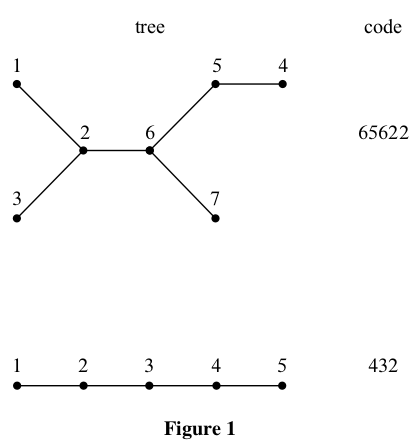
\includegraphics[scale=0.5]{numbered-tree.png}
\end{figure}

\subsection{(a)}
Describe a procedure for reconstructing a numbered tree from its code.
\begin{proof}
The key observation is that, given a code of length $n - 2$, the numbers between $1$ and $n$ which do not appear in the code are precisely the leaves of the tree. This follows because the vertices
left at the end of the process are both leaves. So the procedure must have changed all the nonleaf vertices into leaves, and this implies that all the nonleaf vertices appear in the code.

Hence, the largest missing number is a leaf attached to the first number of the code. The rest of the tree can now be reconstructed by deleting the first number in the code, henceforth ignoring the largest leaf, and proceeding recursively on the rest of the code. (We’re using the obvious fact that what’s left after deleting a leaf from a tree is another tree.)

More precisely, the reconstruction procedure applies to any finite tree whose vertex set is totally ordered. The procedure takes two parameters: the vertex set, $V$, and a length $|V| - 2$ “code”
sequence, $S$, of elements in $V$. If $l$ is the largest element in $V$ which does not appear in $S$, and $f$ is the first element of $S$, then the reconstructed tree is obtained by adding edge $(l, f)$ to the tree reconstructed by calling the procedure recursively with first argument $V - \{l\}$ and second argument equal to the code obtained by erasing the initial f from S. The procedure terminates when $|V| = 2$, returning the edge between the two numbers in $V$.
\end{proof}

\subsection{(b)}
Conclude there is a bijection between the $n$-vertex numbered trees and $\{1, \ldots, n\}^{n-2}$, and state how many $n$-vertex numbered trees there are.
\begin{proof}
There are exactly as many $n$-vertex numbered trees as the number of possible code words, that is, the number of length $n - 2$ sequences of integers between 1 and n. So there are $n^{n-2}$ numbered trees.

The reason is that the map from trees to codes is a bijection. To see this, note that the tree re­construction procedure finds the only possible tree with that code. So there can’t be two trees with
the same code, that is, the map from a tree to its code is an injection. But since the reconstruc­tion procedure finds a tree for every possible codeword, the map from trees to codes is also a
surjection.
\end{proof}

\section{Problem 3}
\subsection{(a)}
Let $S_{n,k}$ be the possible nonnegative integer solutions to the inequality
$$
x_1 + x_2 + \ldots + x_k \leq n
$$
That is:
$$
S_{n,k} \Coloneqq \{(x_1, \ldots, x_k) \in \mathbb{N}^k\,\,\,|\,\,\,x_1 + x_2 + \ldots + x_k \leq n\}
$$
Describe a bijection between $S_{n,k}$ and the set of binary strings with $n$ zeroes and $k$ ones.
\begin{proof}
The notation $0^x$ indicates a length $x$ string of 0’s. The bijection is given by:
$$
(x_1, \ldots, x_k) \longleftrightarrow 0^{x_1}10^{x_2}1\ldots0^{x_k}10^{n-s}
$$
where $s \Coloneqq \sum_{i=1}^{k}x_i$.
\end{proof}

\subsection{(b)}
Let $L_{n,k}$ be the length $k$ weakly increasing sequences of nonnegative integers $ \leq n$. That is
$$
L_{n,k} \Coloneqq \{(y_1, \ldots, y_k) \in \mathbb{N}^k\,\,\,|\,\,\,y_1 \leq y_2 \leq \ldots \leq y_k \leq n\}
$$
Describe a bijection between $L_{n,k}$ and $S_{n,k}$.
\begin{proof}
The bijection is given by, $L_{n,k} \to S_{n,k}$:
$$
(y_1, \ldots, y_k) \longleftrightarrow (y_1, y_2 - y_1, y_3 - y_2, \ldots, y_k - y_{k-1})
$$
In the other direction, $S_{n,k} \to L_{n,k}$:
$$
(x_1, \ldots, x_k) \longleftrightarrow (x_1, x_1+x_2, x_1+x_2+x_3, \ldots, \sum_{i=1}^{k}x_i)
$$
\end{proof}

\section{Problem 4 (Supplemental Problem)}
Let $X$ and $Y$ be finite sets.

\subsection{(a)}
How many binary relations from $X$ to $Y$ are there?

\begin{proof}
A binary relation $R: X \to Y$ is a set of pairs $(x,y)$ where $x \in X$ and $y \in Y$. In other words $R \subseteq X \times Y$. So the number of such relations is equal to the number of subsets of the cartesian product $X \times Y$, which is $2^{|X|\cdot|Y|}$.
\end{proof}

\subsection{(b)}
Define a bijection between the set $[X \to Y]$ of all total functions from $X$ to $Y$ and the set $Y^{|X|}$. (Recall $Y^n$ is the Cartesian product of $Y$ with itself $n$ times.) Based on that, what is $|[X \to Y]|$?
\begin{proof}
Assume $X$ has size $n\geq 0$. Let $X = \{x_1, \ldots, x_n\}$ be an enumeration of the elements of $X$. 

Now any total function $f: X \to Y$ is uniquely determined by the values\\ $f(x_1),  \ldots, f(x_n)$ which are elements of $Y$.

So the bijection is:
$$
f \longleftrightarrow (f(x_1), \ldots, f(x_n)) \in Y^n
$$

Based on the bijection, $|[X \to Y]| = |Y^{|X|}| = |Y|^{|X|}$.
\end{proof}

\subsection{(c)}
Using the previous part, how many functions, not necessarily total, are there from $X$ to $Y$? How does the fraction of functions vs. total functions grow as the size of $X$ grows? Is it $O(1), O(|X|), O(2^{|X|}), \ldots$?
\begin{proof}
Again, assume $X$ has size $n\geq 0$. Let $X = \{x_1, \ldots, x_n\}$ be an enumeration of the elements of $X$. 

By using the same idea as in the previous part, we can also calculate the number of partial functions $f: X \to Y$.

For example, if $f$ is defined on 0 elements of $X$, then we see that there are $|Y|^0 = 1$ such partial functions.

If $f$ is defined on exactly 1 element of $X$, then we see that there are $n \cdot |Y|^1 = 1$ such partial functions. Why is it multiplied by $n$? Well, $f$ could be defined only on $x_1$, or $f$ could be defined only on $x_2$, and so on. For each such choice, the output has $|Y|$ choices.

Similarly, if $f$ is defined exactly on 2 elements of $X$, then there are $\binom{n}{2}\cdot |Y|^2$ such functions (there are $\binom{n}{2}$ ways to choose the 2 elements of $X$ on which $f$ is defined; for each such choice there are $|Y|^2$ ways to choose their outputs).

So, generalizing this, we see that the number of all functions, partial or total, is:
$$
\sum_{i = 0}^n \binom{n}{i}|Y|^i
$$
By the Binomial Theorem this is equal to $(1+|Y|)^n$. Remember that $n = |X|$, so this is $(1+|Y|)^{|X|}$.

The fraction of all functions vs total functions is:
$$
\frac{(1+|Y|)^{|X|}}{|Y|^{|X|}}
$$
Assuming $|Y| \geq 1$ is a fixed constant integer, this fraction is $O\left(\left(\frac{1+|Y|}{|Y|}\right)^{|X|}\right)$.
\end{proof}

\subsection{(d)}
Show a bijection between the powerset, pow$(X)$, and the set $[X \to \{0,1\}]$ of 0-1-valued total functions on $X$.
\begin{proof}
Again, assume $X$ has size $n\geq 0$. Let $X = \{x_1, \ldots, x_n\}$ be an enumeration of the elements of $X$. 

Now any subset $S$ of $X$ is uniquely determined by whether or not it contains each $x_i$. We can uniquely represent this with a sequence of 0's and 1's. In the $i$th digit of the sequence, a 0 corresponds to $S$ not containing $x_i$, whereas a 1 corresponds to $S$ containing $x_i$.

For example, if $X = \{x_1, x_2, x_3\}$ and the subset $S$ is $S = \{x_1, x_3\}$ then the unique sequence representing $S$ is 101.

In other words, for each subset $S \subseteq X$, this sequence defines a total function $f_S : X \to \{0,1\}$ defined by:
$$
f_S(x) \Coloneqq 1 \text{ if } x \in S, \,\,\, 0 \text{ if } x \notin S.
$$
The bijection from pow$(X)$ to $[X \to \{0,1\}]$ is given by $S \longleftrightarrow f_S$.
\end{proof}

\subsection{(e)}
Let $X$ be a set of size $n$ and $B_X$ be the set of all bijections from $X$ to $X$. Describe a bijection from $B_X$ to the set of permutations of $X$. This implies that there are how many bijections from $X$ to $X$?
\begin{proof}
Let $X = \{x_1, \ldots, x_n\}$ be an enumeration of the elements of $X$. 

Any bijection $f: X \to X$ is determined by what it does to each input $x_i$. In other words, $f$ is determined by the values $f(x_1), \ldots, f(x_n)$.

These values $f(x_i)$ are also elements of $X$ (because $f: X \to X$), so each $f(x_i)$ is equal to some $x_j$. 

Since $f$ is total, it takes all $n$ different inputs $x_1, \ldots, x_n$; and since $f$ is a bijection, it takes on each of the $n$ possible different outputs $x_1, \ldots, x_n$ exactly once. So $f$ is simply permuting the elements $x_1, \ldots, x_n$ of $X$.

For example if $X = \{x_1, x_2, x_3\}$ one possible bijection is defined by the permutation: 
$$
\begin{array}{ccc}
f(x_1) &=& x_3\\ 
f(x_2) &=& x_1\\ 
f(x_3) &=& x_2
\end{array}
$$
So there is a bijection between $B_X$ and the set of all permutations of $X$. This implies that there are $n!$, or, $|X|!$ bijections from $X$ to $X$.
\end{proof}

\end{document}























